\documentclass{article}


% Things to import:
\usepackage{tikz}



\begin{document}
% Used to export it as an image too: (Sourcecode is from here: https://tex.stackexchange.com/a/299008)
\hoffset=-1in\voffset=-1in\setbox0\vbox{


\centering
	
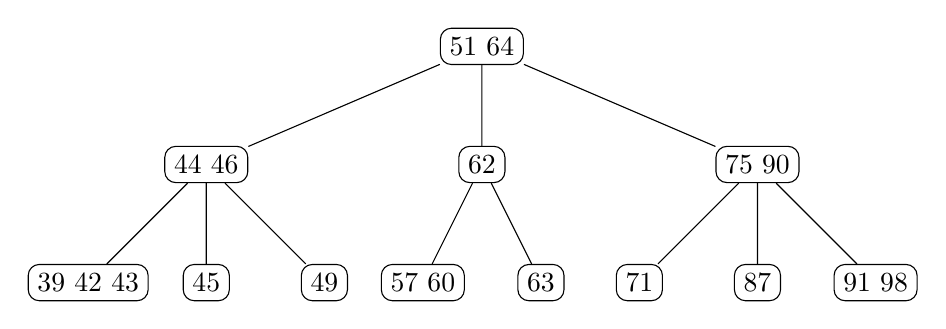
\begin{tikzpicture}
[every node/.style={shape=rectangle,rounded corners,draw,align=center},
level 1/.style={sibling distance=35mm},
level 2/.style={sibling distance=15mm}]

\node {51 64}
child { node {44 46}
	child { node {39 42 43}}
	child { node {45}}
	child { node {49}}
}
child { node {62}
	child { node {57 60}}
	child { node {63}}
}
child { node {75 90}
	child { node {71}}
	child { node {87}}
	child { node {91 98}}
}
;
\end{tikzpicture}

\bigbreak

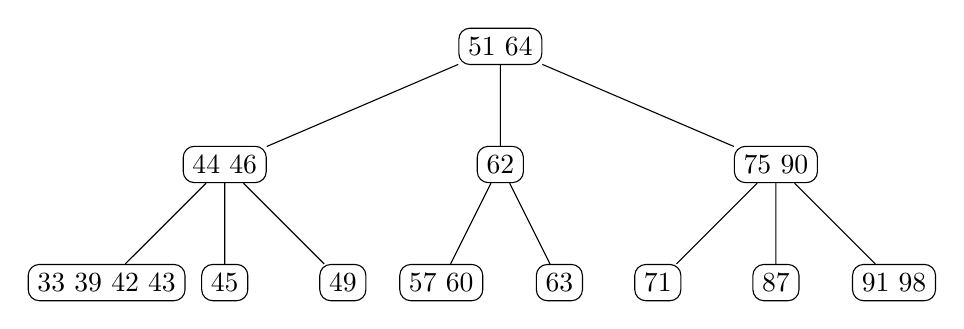
\begin{tikzpicture}
[every node/.style={shape=rectangle,rounded corners,draw,align=center},
level 1/.style={sibling distance=35mm},
level 2/.style={sibling distance=15mm}]

\node {51 64}
child { node {44 46}
	child { node {33 39 42 43}}
	child { node {45}}
	child { node {49}}
}
child { node {62}
	child { node {57 60}}
	child { node {63}}
}
child { node {75 90}
	child { node {71}}
	child { node {87}}
	child { node {91 98}}
}
;
\end{tikzpicture}

\bigbreak

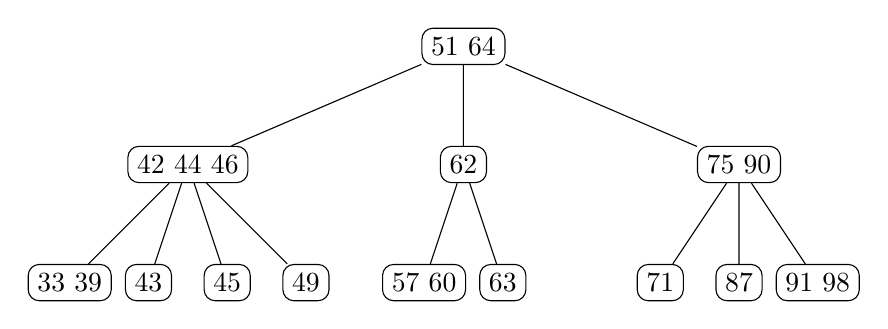
\begin{tikzpicture}
[every node/.style={shape=rectangle,rounded corners,draw,align=center},
level 1/.style={sibling distance=35mm},
level 2/.style={sibling distance=10mm}]

\node {51 64}
child { node {42 44 46}
	child { node {33 39}}
	child { node {43}}
	child { node {45}}
	child { node {49}}
}
child { node {62}
	child { node {57 60}}
	child { node {63}}
}
child { node {75 90}
	child { node {71}}
	child { node {87}}
	child { node {91 98}}
}
;
\end{tikzpicture}

	
}\pdfpageheight=\dimexpr\ht0+\dp0\relax\pdfpagewidth=\wd0\shipout\box0\stop